\documentclass[10pt]{article}
\usepackage{../../local}
\urlstyle{same}

\newcommand{\classcode}{Physics 110B}
\newcommand{\classname}{Electromagnetics and Optics II}
\renewcommand{\maketitle}{%
\hrule height4pt
\large{Eric Du \hfill \classcode}
\newline
\large{HW 01} \Large{\hfill \classname \hfill} \large{\today}
\hrule height4pt \vskip .7em
\small{Header styling inspired by Berkeley EECS Department: \url{https://eecs.berkeley.edu/}}
\normalsize
}
\linespread{1.2}
\begin{document}
	\maketitle
	\section*{Problem 1}
	In a compact region \( \mathcal{V} \) surrounded by the surface \( \mathcal{S} \), we have a
	time-dependent charge density \( \rho(t, \mathbf{r}) \) moving in the electromagnetic field \(
	\mathbf{E}(t, \mathbf{r}) \) and \( \mathbf{B}(t, \mathbf{r}) \).
	\begin{enumerate}[label=(\alph*)]
		\item Show that the time changing rate of field energy \( \displaystyle\int_{\mathcal{V}}\left(
			\frac{\epsilon_0}{2}|\mathbf{E}|^2 + \frac{1}{2\mu_0}|\mathbf{B}|^2 \right) \diff \tau \) is
			equal to the negative flux (energy transferred per unit time) passing through the surface \(
			\mathcal{S} \). In other words, prove the Poynting theorem starting from
			\[
				\dv{W}{t} = \int_{\mathcal{V}}(\mathbf{E} + \mathbf{v} \times \mathbf{B}) \cdot \mathbf{v}
				\rho \diff \tau
			\]
			where \( dW \) is the work done on the charge density by the electric and magnetic field,
			and \( \mathbf{v} \) is the velocity of the charge distribution.  

			\begin{center}
				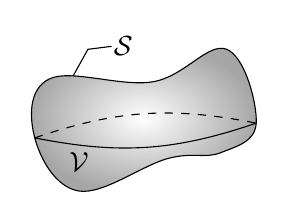
\begin{tikzpicture}[scale=0.75]
					\draw[inner color=white, outer color=gray!70] plot [smooth cycle, tension = 0.65] coordinates {
						(0,0)
						(0.25,1)
						(2,0.95)
						(3.25,1.5)
						(3.75,0.25)
						(3.15,-0.25)
						(2.25,-0.35)
						(0.75,-0.9)};
					\node at (1.5,1.55) {$\mathcal{S}$};
					\draw (0,0) to[bend right=15] (3.75,0.25) node[below,xshift=-2.25cm,yshift=-0.25cm] {$\mathcal{V}$};
					\draw[dashed] (0,0) to[bend left=15] (3.75,0.25);
					\draw (0.65,1.05) -- (0.9,1.5) -- (1.3,1.55);
			\end{tikzpicture}
			\end{center}

			\begin{solution}
				We follow the same derivation as the one we did in class. First, we start by noticing that \(
				(\mathbf{v} \times \mathbf{B})\cdot \mathbf{v} = \mathbf{0}\), as the cross product produces
				a vector perpendicular to \( \mathbf{v} \). As such, the equation immediately simplifies to
				\[
					\dv{W}{t} = \int_{\mathcal{V}} \mathbf{E} \cdot \mathbf{v} \rho \diff \tau =
					\int_{\mathcal{ V}}\mathbf{J} \cdot \mathbf{E} \diff \tau 
				\]
				utilizing the relation \( \rho \mathbf{v} = \mathbf{J} \). Now, we use Ampere-Maxwell
				equation to rewrite this equation purely in terms of \( \mathbf{B} \) and \( \mathbf{E} \):
				\[
					\dv{W}{t} = \int_{\mathcal{V}} \left( \frac{1}{\mu_0}(\curl \mathbf{B}) - \epsilon_0
					\partial_t \mathbf{E}) \cdot \mathbf{E} \right) = \int_\mathcal{V} \frac{1}{\mu_0}(\curl
					\mathbf{B}) \cdot \mathbf{E} \diff \tau - \int_{\mathcal{V}}\epsilon_0 (\partial_t
					\mathbf{E}) \cdot \mathbf{E} \diff \tau
				\]
				Now we deal with each term separately. We can simplify the second term using product rule:
				\[
					\int_{\mathcal{V}} \epsilon_0 (\partial_t \mathbf{E}) \cdot \mathbf{E} \diff \tau =
					\frac{1}{2}\int_\mathcal{V} \epsilon_0 \partial_t(\mathbf{E} \cdot \mathbf{E}) \diff \tau
					= \dv{t} \int_{\mathcal{V}} \frac{\epsilon_0}{2}|\mathbf{E}|^2 \diff \tau
				\]
				Now for the first term. We use index notation to simplify it down:
				\begin{align*}
					(\curl \mathbf{B}) \cdot \mathbf{E} &= \epsilon^{ijk}(\partial_j B_k) E_i = \epsilon^{ijk} \partial_j (B_k
					E_i) - \epsilon^{ijk}B_k (\partial_j E_i)\\
					&= -\epsilon^{ijk}\partial_j (B_k E_i) - \epsilon^{kij}B_k(\partial_j E_i) \\ 
					&= -\epsilon^{ijk}\partial_j (B_k E_i) + \epsilon^{kji} B_k (\partial_j E_i) 
				\end{align*}
				Note that the Levi-Civita tensor \( \epsilon^{ijk} \) does not change under cyclic permutations of summation,
				but changes sign when we perform a swap of two adjacent indices. Now, the first term gives \( \div(\mathbf{E}
				\times \mathbf{B})\), and the second term gives \( \mathbf{B} \cdot (\curl \mathbf{E}) \). So, the first
				integral becomes:
				\[
					-\frac{1}{\mu_0} \int_{\mathcal{V}} \div(\mathbf{E} \times \mathbf{B}) \diff \tau +
					\frac{1}{\mu_0}\int_{\mathcal{V}} \mathbf{B} \cdot (\curl \mathbf{E}) \diff \tau 
				\]
				Now finally, we can use Faraday's law to write \( \curl \mathbf{E} = -\partial_t
				\mathbf{B} \), which in the second term allows you to write it as \( \frac{1}{2\mu_0}|\mathbf{B}|^2 \).
				Simultaneously, we use divergence theorem on the first term to write it as a surface integral:  
				\[
					-\frac{1}{\mu_0} \oint_{\partial \mathcal{V}}(\mathbf{E} \times \mathbf{B}) \diff \mathbf{a} +
					\frac{1}{\mu_0} \int_{\mathcal{V}} \mathbf{B} \cdot (-\partial_t \mathbf{B}) \diff \tau =
					-\frac{1}{\mu_0}\oint_{\partial \mathcal{ V}}(\mathbf{E} \times \mathbf{B}) \diff \mathbf{a} - \dv{t}
					\int_{\mathcal{V}}\left( \frac{1}{2\mu_0} |\mathbf{B}|^2\right) \diff \tau 
				\]
				Now, we can put this all together:
				\[
					\dv{W}{t} = -\frac{1}{\mu_0} \oint_{\partial \mathcal{V}} (\mathbf{E} \times \mathbf{B}) \diff
					\mathbf{a} - \dv{t} \int_{\mathcal{V}}\left( \frac{1}{2\mu_0}|\mathbf{B}|^2 +
					\frac{\epsilon_0}{2}|\mathbf{E}|^2 \right) \diff \tau 
				\]
				Moving the first term to the left hand side:
				\[
					\dv{W}{t} + \dv{t} \int_{\mathcal{V}}\left( \frac{1}{2\mu_0}|\mathbf{B}|^2 +
					\frac{\epsilon_0}{2}|\mathbf{E}|^2 \right)\diff \tau = -\frac{1}{\mu_0}\oint_{\partial
					\mathcal{V}}(\mathbf{E} \times \mathbf{B}) \diff \mathbf{a}
				\]
				This is the Poynting theorem, as desired. The integral on the right side is a flux integral,
				and the second quantity on the left hand side is the rate of change of the field energy.
			\end{solution}
	\end{enumerate}
	radius \( R \) and length \( L \). There is a \textit{uniform} steady (i.e. time-independent) current
	density \( \mathbf{J} \) flowing in the axial direction as shown in the right figure. We assume the
	material satisfies Ohm's law, and it's only the static electric field inside the material that is
	responsible for pushing the current. We also assume the entire segment, including both the surface and
	the volume are electrically neutral, i.e. there are no volume or surface charge densities.
	\begin{center}
		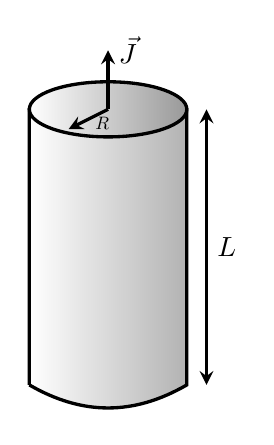
\begin{tikzpicture}
			\draw[very thick, left color=white,right color=gray!60!white] 
				(-1,-1.75) -- (-1,1.75) to[bend left=25] (1,1.75) -- (1,-1.75) to[bend left=30] (-1,-1.75);
			\foreach \pos in {(0,1.75)} {
				\draw[very thick, left color=white, right color=gray!80] \pos ellipse (1cm and 0.35cm);
			}
			\draw[stealth-stealth,very thick] (1.25,-1.75) -- (1.25,1.75) node[midway,right] {$L$}; 
			\draw[very thick,-stealth] (0,1.75) -- (-0.5,1.5) node[midway, right,yshift=-0.05cm,scale=0.65] {$R$};
			\draw[very thick,-stealth] (0,1.75) -- (0,2.5) node[right] {$\vec{J}$};
		\end{tikzpicture}
	\end{center}
	\begin{enumerate}[label=(\alph*), resume]
		\item Show that the electric field right outside the wire, i.e. \( s = R^{+} \) is equal to the
			electric field inside the wire. 

			\begin{solution}
				Becuase the conductor follows Ohm's law, we know that \( \mathbf{J} = \sigma \mathbf{E} \),
				and hence the \( \mathbf{E} \) field is uniform inside the cylinder. Then, we know that
				along boundaries, we have the following equation:
				\[
					\mathbf{E}^{\parallel}_\text{above} - \mathbf{E}^{\parallel}_{\text{below}} = \mathbf{0}
				\]
				in other words, if we consider the boundary of the cylinder, then this equation directly 
				tells us that the electric field right outside the wire is equal to the electric field inside
				the wire. 

				Likewise, for the perpendicular segment: we notice that there are no surface charges anywhere, so
				this means that:
				\[
					E^{\perp}_\text{above} - E^{\perp}_\text{below} = 0
				\]
				this implies that the magnitude of the \( \mathbf{E} \) field perpendicular to the cylinder
				should be the same in magnitude as well. There is obviously no \( \mathbf{E}  \) field in the
				\( \hat{\phi} \) direction (both outside and inside the wire) due to symmetry, 
				so checking these three conditions implies that
				the \( \mathbf{E} \) field just outside the wire is equal to that inside the wire. 
			\end{solution}
		\item Find the energy flux through the side surface of the wire. Does the energy flow into or out of
			the wire?

			\begin{solution}
				To do this, we find the Poynting vector \( \mathbf{S} = \frac{1}{\mu_0}(\mathbf{E} \times
				\mathbf{B}) \). We already have \( \mathbf{E} \) from \( \mathbf{J} \), so all we need to
				figure out is \( \mathbf{B} \). From Ampere's law, consider a loop of radius \( r \) centered
				around the center of the cylinder. Because \( \mathbf{J} \) is uniform, then we conclude that
				the flux through the Amperian loop is also uniform, and hence:
				\[
					\oint \mathbf{B} \cdot \diff \mathbf{l} = |\mathbf{B}|(2 \pi r) = \mu_0 I_\text{enc}
				\]
				The enclosed current is given by \( \int \mathbf{J} \cdot \diff \mathbf{a} = |\mathbf{J}| \pi
				r^2	\), so the equation now reads:
				\[
					|\mathbf{B}| (2 \pi r) = \mu_0 |\mathbf{J}| \pi r^2 \implies |\mathbf{B}| = \frac{\mu_0
					|\mathbf{J}|r}{2}
				\]
				Now, since \( \mathbf{J} \) points in the \( \mathbf{\hat{z}} \) direction, then by the right hand
				rule we know that \( \mathbf{B} \) points in the \( \boldsymbol{\hat{\phi}} \) direction.
				Finally, we can calculate \( \mathbf{S} \) (while using \( \mathbf{B} \) 
				at \( r = R \) to cover the entire wire):
				\[
					\mathbf{S} = \frac{1}{\mu_0\sigma} \frac{\mu_0 |\mathbf{J}| R}{2} \mathbf{J} \times
					\boldsymbol{\hat{\phi}} = -\frac{|\mathbf{J}|^2R}{2 \sigma}\mathbf{\hat{r}}
				\]
				The flux is then \( \displaystyle \Phi_{S} = \oint \mathbf{S} \cdot \diff \mathbf{a} \), 
				and due to the uniformity of \( \mathbf{S} \) this is just \( \mathbf{S} \) 
				multiplied by the surface area of the wire, so:
				\[
					\Phi_S = -\frac{JR}{2 \sigma} (2 \pi R L) = -\frac{\pi |\mathbf{J}|^2R^2 L}{\sigma}
				\]
				The flux is negative to indicate that the flux flows into the wire -- this is a result of \(
				\mathbf{S}\) pointing in the \( -\mathbf{\hat{r}} \) direction. 

				Initially, I was quite disturbed by this fact: it seems that the Poynting vector indicates
				that the energy used to move the charges is coming from thin air. This seems
				counter-intuitive at first, but the way to reconcile this is to realize that the \(
				\mathbf{S} \) field exists across all space (since \( \mathbf{E} \) and \( \mathbf{B} \) do),
				so when power is being dissipated by the wire segment, energy flows from the fields into the
				wire, so that energy is conserved. So, the energy is not actually coming from thin air, but
				rather from the invisible electromagnetic fields that exist everywhere. It should also be
				mentioned that the only way for this system to be physical is if it is hooked up to a battery
				-- otherwise having \( \mathbf{J} \) flow into a wall that doesn't accept surface charges is
				completely nonphysical. 
			\end{solution}
		\item Calculate the power done on the net current flowing in that segment by the electric force.

			\begin{solution}
				The power is given by:
				\[
					\dv{W_\text{EM}}{t} = \int_{\mathcal{V}} \mathbf{J} \cdot \mathbf{E} \diff \tau =
					\int_{\mathcal{V}} \sigma \mathbf{E} \cdot \mathbf{E} \diff \tau
				\]
				Now, \( \mathbf{E} \cdot \mathbf{E} = |\mathbf{E}|^2 = \frac{|\mathbf{J}|^2}{\sigma^2} \).
				The quantity is also constant over the volume, so this integral becomes:
				\[
					\int_{\mathcal{V}} \sigma |\mathbf{E}|^2 \diff \tau = \sigma
					\frac{|\mathbf{J}|^2}{\sigma^2} \pi R^2 L = \frac{\pi |\mathbf{J}|^2 R^2 L}{\sigma}
				\]
				This is a good sign, because its exactly negative in magnitude to the answer we got in (c).  
			\end{solution}
	\end{enumerate}
	Note that your answer in part (c) and (d) should be equal to each other, as stated by the Poynting
	theorem. 

	\pagebreak
	\section*{Problem 2}
	A point charge of charge \( +q \) is located at \( (a, 0, 0) \) at rest, and another point charge of
	charge \( -q \) is located at \( (-a, 0, 0) \) at rest. The two point charges are immersed in a uniform
	magnetic field \( \mathbf{B} = B \hat{\mathbf{z}} \).
	\begin{enumerate}[label=(\alph*)]
		\item Prove that the streamlines of the Poynting vector \( \mathbf{S} \) either close on themselves
			or begin and end at infinity. \textit{Hint: For a vector field like this, should it be
			divergenceless, or curl-less?}

			\begin{solution}
				To prove this, we consider \( \div (\mathbf{E} \times \mathbf{B}) \). From the vector product
				rule, we know that this is equal to:
				\[
					\div(\mathbf{E} \times \mathbf{B}) = \mathbf{B} \cdot (\curl \mathbf{E}) - \mathbf{E}
					\cdot (\curl \mathbf{B})
				\]
				From Faraday's law, we know that \( \curl \mathbf{E} = -\partial_t \mathbf{B} \), and since
				the \( \mathbf{B} \) field is static in this problem, then this term is zero. Then, the
				Ampere-Maxwell law says that \( \curl \mathbf{B} = \mu_0 \mathbf{J} + \mu_0 \epsilon_0
				\partial_t \mathbf{E} \). The system here is completely static so there is no current density
				\( \mathbf{J} \), and the \( \mathbf{E} \) field is static, so this term is also zero. Thus, 
				we can only conclude:
				\[
					\div(\mathbf{E} \times \mathbf{B}) = \mathbf{0}
				\]
				and hence the Poynting vector is divergenceless. To show that it must not be curl-less we can
				leverage two facts simultaneously: first, we know that \( \mathbf{S} \) must be nonzero,
				since there exists a nonzero, and non-parallel \( \mathbf{E} \) and \( \mathbf{B} \) field.
				Further, \( \mathbf{S} \) must be smooth as there are no discontinuities besides possibly the
				charges themselves. Thus, we can use the Helmholtz theorem to conclude that the only
				resolution to this is the fact that \( \mathbf{S} \) cannot be curl-less, since a curl-less
				\( \mathbf{S} \) would imply that \( \mathbf{S} \) is zero everywhere. As such, the \(
				\mathbf{S} \) field must close in on itself. 

				EDIT: I later found out that this approach actually doesn't suffice, because you can have a
				vector field which is divergenceless and curlless. However, I believe that if you add the
				condition that the field is \textit{nonconstant}, then the theorem does hold. In our case,
				the \( \mathbf{S} \) field is clearly nonconstant, so in light of this I do believe my
				approach does work.  
			\end{solution}
		\item Sketch several representative field lines of the Poynting vector \( \mathbf{S}(x, y) \) on the
			\( xy \)-plane, including the one that passes through the origin of the coordinate system.
			\textit{Note: You should find that the net Poynting flux towards the charges to be zero. This
				makes sense because the particles are at rest, and thus the power done on the particles by
			the electromagnetic force is zero.}

			\begin{solution}
				Drawing out the electric field lines, it's clear that between \( x \in (-a, a) \), the \(
				\mathbf{E} \) field lines travel from the positive to the negative charge. As such, \(
				\mathbf{E} \) points in the \( -\hat{\mathbf{x}} \) direction. Then, outside of this region,
				the \( \mathbf{E} \) points in the \( -\hat{\mathbf{x}} \) direction on the right, and in the
				\( +\hat{\mathbf{x}} \) direction on the left. And, since the \( \mathbf{S} \) vector forms
				loops in this case, it is reasonable to extrapolate that the \( \mathbf{S} \) vector forms
				loops around both charges, clockwise around \( +q \) and anti-clockwise around \( -q \). 

				For the line going through the origin, we know that \( \mathbf{E} \) is purely in the \(
				-\hat{\mathbf{x}} \) direction, which means that the Poynting vector points only in the \(
				\hat{\mathbf{y}} \) direction. 

				I drew a diagram on a blackboard:
				\begin{center}
					\includegraphics[scale=0.05]{2b.jpg}
				\end{center}
				Yeah it's not that pretty but I also CANNOT be bothered right now to try and render this in
				latex. 
			\end{solution}
	\end{enumerate}


	\pagebreak
	\section*{Problem 3}
	\begin{enumerate}[label=(\alph*)]
		\item Consider two equal point charges \( q \), separated by a distance \( 2a \). Construct the plane
			equidistant from the two charges. By integrating Maxwell's stress tensor over this plane,
			determine the force of one charge on the other.

			\begin{solution}
				By the symmetry of the problem, the \( \mathbf{E} \) field in the plane has no 
				\( \hat{\mathbf{z}} \) component. Using cylindrical coordinates, the \( \mathbf{E} \) field
				can be written as
				\[
					\mathbf{E} = \frac{2kq}{R^2} \sin \theta \hat{\mathbf{r}}
				\]
				the factor of 2 exists because there are two charges present, and the \( \sin \theta \) is
				there to pick out the horizontal component of the \( \mathbf{E} \) field. Now, the Maxwell
				stress tensor is:
				\[
					T_{ij} = \epsilon_0 \left(E_i E_j - \frac{1}{2}|\mathbf{E}|^2\right) +
					\frac{1}{2\mu_0}\left( B_iB_j - \frac{1}{2}|\mathbf{B}|^2 \right)
				\]
				There is no \( \mathbf{B} \) field in this problem, so that entire term is zero. Now, \(
				T_{x x} \) and \( T_{yy} \) must also be zero, due to the symmetry in the problem. Therefore,
				we only need to calculate \( T_{zz} \). \( E_z = 0 \) as mentioned earlier, so
				\[
					T_{zz} = -\frac{\epsilon_0}{2} |\mathbf{E}|^2
				\]
				Using \( \mathbf{E} \) from earlier, we have:
				\[
					|\mathbf{E}|^2 = \frac{4 k^2 q^2}{R^{4}} \sin^2 \theta
				\]
				From the geometry of the problem (see diagram), we have \( \sin \theta = \frac{r}{R} \), so
				\[
					|\mathbf{E}|^2 = \frac{4k^2 q^2}{R^{4}}\left( \frac{r^2}{R^2} \right) =
					\frac{4k^2q^2r^2}{(a^2 + r^2)^3}
				\]
				So \( T_{zz} \) is:
				\[
					T_{zz} = -\frac{\epsilon_0}{2}\frac{4k^2q^2r^2}{(a^2 + r^2)^3}
				\]
				Finally, we can integrate this over the entire plane. Using polar coordinates, we have:
				\begin{align*}
					\mathbf{F} = \oint_{\mathcal{S}}T_{zz}\diff \mathbf{a}_z &=
					\int_{0}^{\infty}\int_{0}^{2\pi} - \frac{\epsilon_0}{2} \frac{4k^2q^2r^2}{(a^2 + r^2)^3}r
					\diff r \diff \theta\\ 
					&= -2k^2q^2 \epsilon_0 (2\pi) \int_{0}^{\infty}\frac{r^3}{(a^2 + r^2)^3} \diff r 
				\end{align*}
				I'm too lazy to do this integral by hand so I plugged it into wolfram, which gave me the
				result:
				\[
					\mathbf{F} = \frac{-4\pi \epsilon_0 k^2 q^2}{4a^2} = -\frac{1}{4 \pi
					\epsilon_0}\frac{q^2}{4a^2}
				\]
			\end{solution}
		\item Do the same for charges that are opposite in sign. 

			\begin{solution}
				Here, \( T_{zz} \) is a bit different because \( E_z \) is nonzero:
				\[
					T_{zz} = \epsilon_0 \left( E_z^2 - \frac{1}{2}|\mathbf{E}|^2 \right)
				\]
				Now, what is nice here is that \( \mathbf{E} \) points strictly in the \( \hat{\mathbf{z}} \)
				direction, so this means that \( |\mathbf{E}| = E_z^2 \), so:
				\[
					T_{zz} = \frac{\epsilon_0}{2} |\mathbf{E}|^2
				\]
				Finally, we can integrate this. Again from the geometry, 
				\[
					|\mathbf{E}|^2 = \frac{4k^2q^2}{R^{4}}\cos^2 \theta = \frac{4k^2q^2a^2}{(a^2 + r^2)^3}
				\]
				We now integrate this over the entire plane:
				\[
					\mathbf{F} = \int_{0}^{\infty}\int_{0}^{2\pi} \frac{\epsilon_0}{2}\frac{4k^2q^2 a^2}{(a^2
					+ r^2)^3} r \diff r \diff \theta 
				\]
				Again, I'm lazy, so:
				\[
					\mathbf{F} = \frac{1}{4\pi \epsilon_0}\frac{q^2}{4a^2}
				\]
				This result also makes sense, as its the same magnitude but opposite sign to the result we
				got from the previous part.  
			\end{solution}
	\end{enumerate}
\end{document}
